\chapter{Methods and Tools for Argumentation Mining of Claims}

%This chapter is divided into three main parts. 
This chapter should be viewed as an overview of most methods used in the rest
of the thesis. Models of argumentation mining are mostly built on machine
learning, which is introduced in section~\ref{sec:unstruc_machine_learning}.
Then, in section~\ref{sec:struc_machine_learning} we focus on a
subarea of machine learning, structured prediction, as it is the foundation of
part~\ref{part:struc}. Next, as argumentation mining is a subarea of 
natural language processing, a brief introduction to the field, along with some
relevant problems will be explained in section~\ref{sec:natural_language_processing}. 
Finally, knowledge represetation relevant to this thesis will be explained in
~\ref{sec:knowledge_representation}. 

\section{Machine Learning}
\label{sec:unstruc_machine_learning}

- machine learning algorithms learn from data \\
- two basic purposes: supervised and unsupervised algorithms \\
- supervised algorithms fit a set of $n$ samples of 
input data $\textbf{X}^n \in \mathbb{R}^n$ to the set of their correponding 
labels $y^n $. When the labels are discrete $y \in \{1, 2, \dots , V\}$ 
supervised learning is called classification (of $V$ classes), 
whereas learning to fit continuous values ($y \in \mathbb{R}$) 
is denoted regression \\

\subsection{Support Vector Machines}
\label{sec:svm}

Support Vector Machines (SVM) \citep{cortes1995support} is one of the most
popular machine learning algorithms. The algorithm has proven useful for many
text-based problems, such as spam classification \citep{drucker1999support},
sentiment analysis \citep{wang2012baselines}, text categorization
\citep{joachims1998text}, and text classification in general
\citep{tong2001support, ikonomakis2005text}. Originally designed as a simple
binary classification procedure, it has been extended to support multiclass
classification \citep{weston1998multi}, structured prediction
\citep{tsochantaridis2005large}, weighted learning \citep{huang2005weighted} and
other. 

Consider a binary classification problem where one has
a training set $S$ consisting of $N$ pairs of examples with assigned labels
$(x_i, y_i)$.

$$
S = \{(x_1, y_1), (x_2, y_2), \dots, (x_N, y_N)\}
$$
where $\forall i, x_i \in \mathbb{R}^d, y_i \in {0, 1}$.
The SVM algorithm first projects the input data $x_i$ to 
higher dimensional space using a 
feature transform function $\phi(x_i)$ then attempts to 
find support vectors which are solutions to the equations:
\begin{align*}
\textbf{w}^T \phi(X) + b = -1 \\
\textbf{w}^T \phi(X) + b = 1
\end{align*}

The solutions to the equations represent margins which divide
the two classes ${-1, 1}$.
The margin width is $\frac{2}{||w||}$. 
To find the weights, one needs to 
optimize for two criteria 
\begin{enumerate*}[label=(\arabic*)]
\item maximize margin width and
\item minimize classification loss
\end{enumerate*} which is done by
$$
\min_{\textbf{w}} \left( \frac{1}{2}||\textbf{w}||^2 + C \sum_{i=1}^{N} \xi_i \right)
$$
where $\xi_i$ is the loss function and $C$ is a parameter of the model.
Typically, \textit{hinge loss} is used as the loss function $\xi_i(x_i, y_i) =
\max(0, 1 - y_i(\textbf{w}^T x_i + b))$ This problem can be solved using
various methods, such as quadratic programming \citep{wu2005svm} or stochastic
optimization \citep{wang2012breaking}.


\subsection{Long short-term memory networks}
\label{sec:lstm}

\begin{figure}
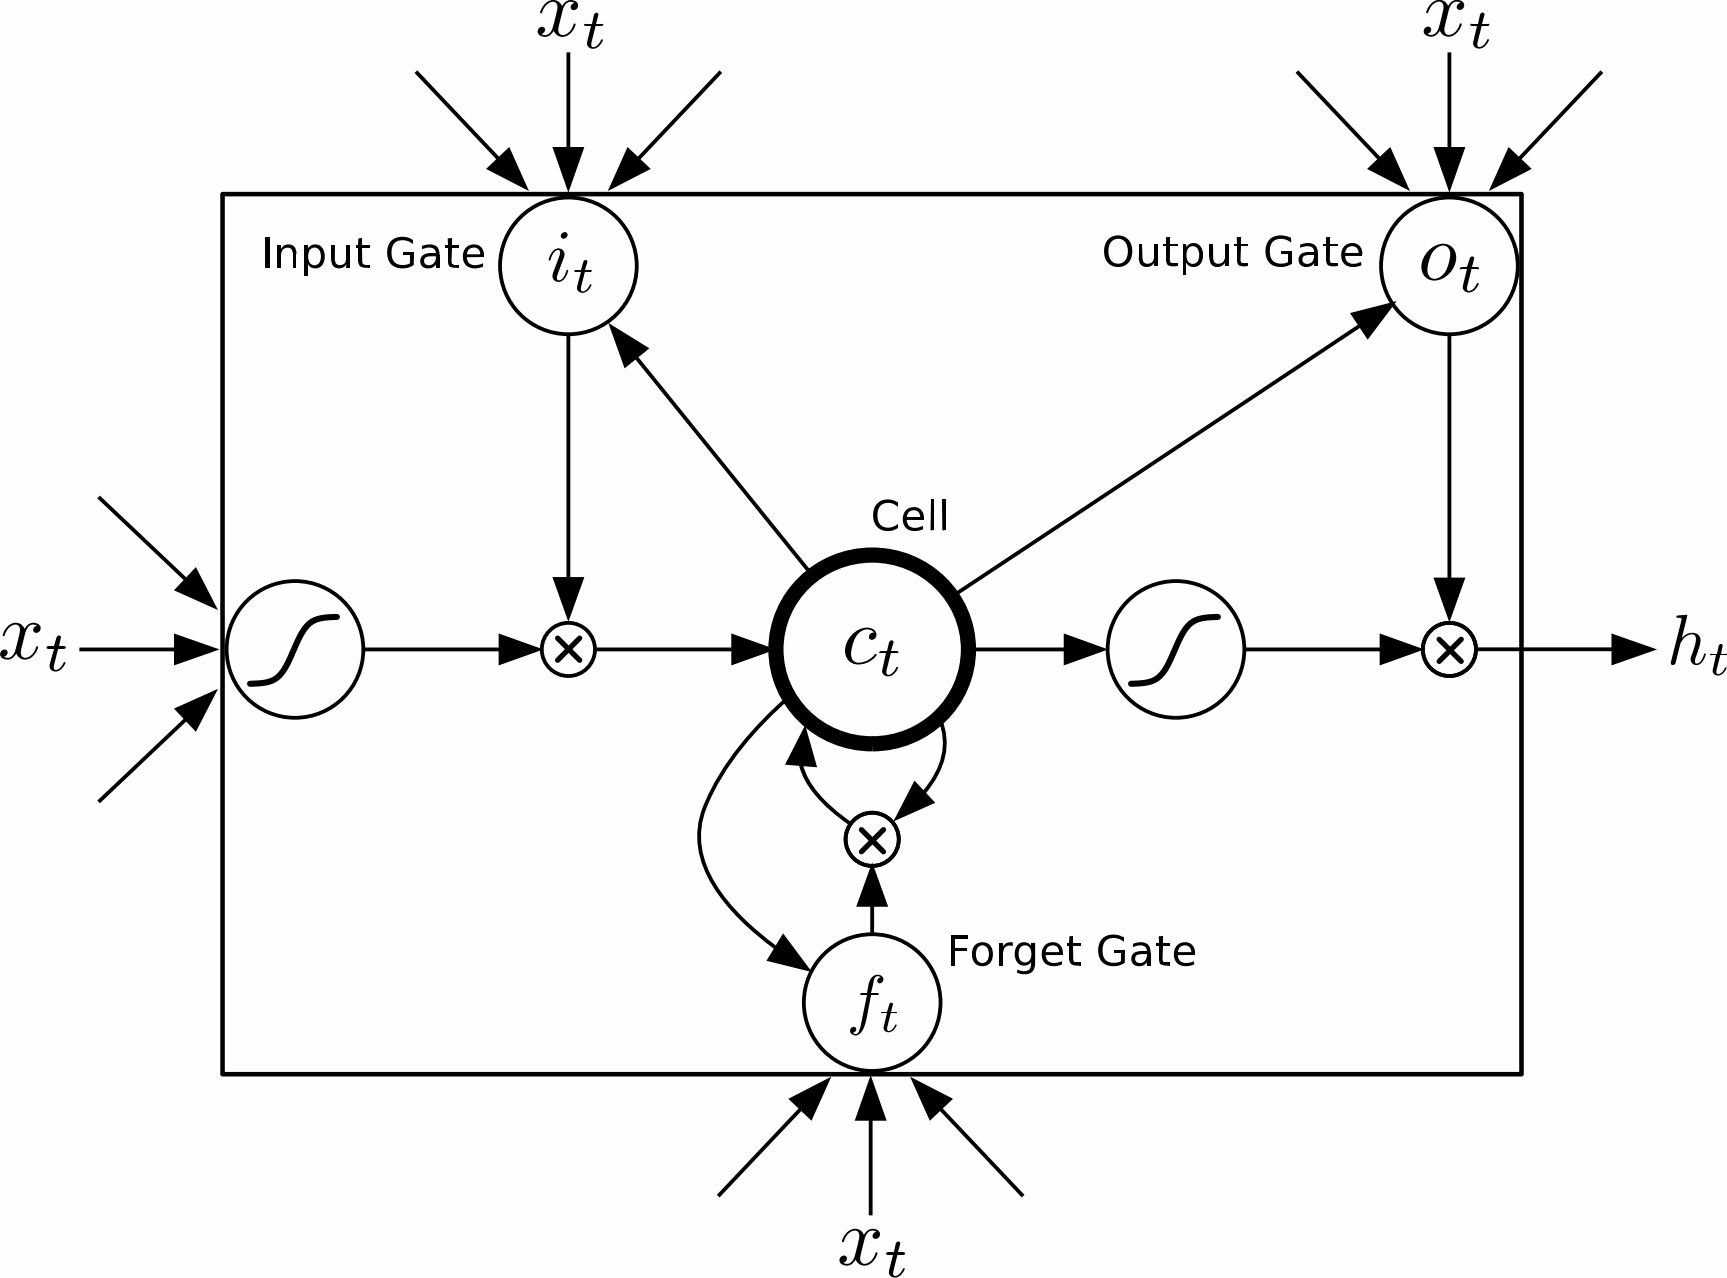
\includegraphics[scale=0.23]{lstm_2.png}
\caption{Long short-term memory network cell diagram. The cell consists of the 
	cell, input gate, forget gate and output gate. The LSTM receives
	the hidden state at the previous time step ($h_{t - 1}$) and $x_t$
	and outputs the hidden state $h_{t}$
	Adopted from 
\citep{graves2013hybrid} }
\label{fig:lstm_arch}
\end{figure}

Long short-term memory (LSTM) is an recurrent neural network
designed to process sequences of data 
\citep{gers1999learning}. A unit of LSTM consists of 
a cell, an input gate, an output gate and a forget gate.
The cell stores information over time intervals and the
gates control which data will be passed on the cell 
or not. Figure \ref{fig:lstm_arch} shows an LSTM cell. 
The input gate ($i$, which new information is going to be stored), 
forget gate ($f$, which information is going to be forgotten from 
the cell state), and output gate ($o$, which is the final output 
of the block) 
are calculated (at timestep $t$) from the input ($\mathbf{x_t}$) and 
previously calculated hidden state ($\mathbf{h_{t-1}}$):
\begin{align*}
	\mathbf{i_t} &= \sigma(\mathbf{w_i} [\mathbf{x_t}, \mathbf{h_{t - 1}}] + b_i) \\
	\mathbf{f_t} &= \sigma(\mathbf{w_f} [\mathbf{x_t}, \mathbf{h_{t - 1}}] + b_f) \\
	\mathbf{o_t} &= \sigma(\mathbf{w_o} [\mathbf{x_t}, \mathbf{h_{t - 1}}] + b_o) \\
\end{align*}
where $\mathbf{w_i, w_f, w_o}$ and $\mathbf{b_i, b_f, b_o}$
are learnable weights of the network and $\sigma$ is the 
sigmoid function ($\sigma(x) = 1 / (1 + e^{-x})$). Next, the 
cell state ($c_t$) and next hidden state ($h_t$) can be calculated as:
\begin{align*}
	\mathbf{\hat{c_t}} &= tanh(\mathbf{w_c} [\mathbf{x_t}, \mathbf{h_{t - 1}}] + b_c) \\
	\mathbf{c_t} &= \mathbf{f_t} \cdot \mathbf{c_{t - 1}} + \mathbf{i_t} \cdot \mathbf{\hat{c_t}} \\
	\mathbf{h_t} &= \mathbf{o_t} \cdot tanh(\mathbf{c_t}) \\
\end{align*}
where $tanh$ represents the hyperbolic tangent function.


The advantage over regular recurrent neural networks, which
don't posses any gating mechanism, is to stop the 
vanishing \citep{hochreiter1998vanishing}
and exploding gradient problems \citep{pascanu2012understanding}. 
The gradients from backpropagation 
can either vanish or explode when training
neural networks causing weight changes to either
stop (vanish) or take on extreme values (explode).
LSTM networks have been successfully applied to a number of problems,
such as language modeling 
\citep{sundermeyer2012lstm}, 
text classification 
\citep{zhou2015c}, question answering 
\citep{zhu2016visual7w}, machine translation
\citep{luong2014addressing}, and many more. LSTM networks are widely considered 
to provide a strong baseline for 
text-based problems. There exist many variations of LSTM networks, 
one example being gated recurrent units (GRU) \citep{chung2014empirical}.

% \subsection{Model Validation}
% 
% Machine learning models are evaluated on unseen data
% to estimate their performance. Traning and testing on the same
% data would lead to overfitting, meaning the model would
% not be able to generalize on new data. 
% To prevent that, 
% data is organized such that 
%  models aren't trained on data they are evaluated on
% (section~\ref{sec:selection})
% after which models are evaluated on unseen data by 
% comparing model predictions versus correct (gold) data
% through various metrics (section ~\ref{sec:metrics})

\subsection{Model Selection}
\label{sec:selection}

The basic model selection method is \textit{holdout}. 
In holdout, the dataset is randomly partitioned into three 
samples: training set (used to train the model), 
validation set (used to assses model performance during training),
and test set (used to asses model performance after training). 

\begin{figure}
	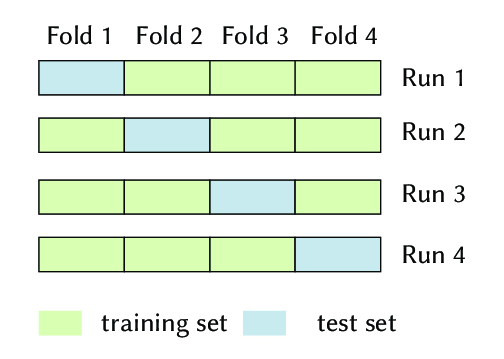
\includegraphics[scale=0.7]{kfold.png}
	\caption{
		Illustration of partitioning a dataset using k-fold model 
	selection using $k = 4$. In each case, $k - 1$ folds
	are used for the training set (green), and the remaining fold is
	the test set (blue). Adopted from \citep{pedregosa2015feature}}
	\label{fig:kfold}
\end{figure}

Another technique to partition datasets into training and test datasets
is cross validation \citep{arlot2010survey} (illustrated in~\ref{fig:kfold})
The training dataset is then used to train the model, and the remaining
test dataset is used to evaluate the resulted trained model. 
\textit{K-fold} cross-validation is the most commonly used
cross-validation technique in which the dataset is partitioned into 
$k$ equally sized samples called folds. One of the $k$ folds is
used as a test dataset, the rest comprise the training dataset. This
procedure is repeated $k$ times (usually $k \in [4, 10] \cap k \in Z$).
Using this method each dataset instance is in the test set 
exactly once. 

In addition to partitioning the data, model selection often involves finding
the optimal hyperparameters of the model, which involves  training and
evaluating the model with a different set of hyperparameters.  Exhaustively
searching through all possible combinations of hyperparameters is called
\textit{grid search} \citep{bergstra2012random}. There are some more advanced
techniques such as \textit{Bayesian optimization}.  For an overview of
hyperparameter optimization techniques see \citep{snoek2012practical}.

\subsection{Evaluation Metrics}
\label{sec:metrics}

Machine learning models are evaluted using metrics to quantify
performance. Supervised classification is more straightforward 
to evaluate and is usually evaluated by calculating  
precision, recall, and f-score. 

In a binary classification setting, we compare bit vectors ($1$ represents the
positive class) of predicted and gold labels. Element-wise comparison will
always give one of four combinations in a confusion matrix (shown in
table~\ref{tab:conf_mat}). Accuracy, precision, recall, and fscore between 
a gold vector $\mathbf{a} = (a_0, a_1, \dots, a_n); \forall i a_i \in \{0, 1\}$ 
and a predicted vector 
$\mathbf{b} = (b_0, b_1, \dots, b_n); \forall i b_i \in \{0, 1\}$
are then defined as:
\begin{align*}
	accuracy(\mathbf{a, b}) &= \frac{TP + TF}{TP + FP + FP + FN} \\
	precision(\mathbf{a, b}) &= \frac{TP}{TP + FP} \\
	recall(\mathbf{a, b}) &= \frac{TP}{TP + FN} \\
	fscore_{\beta}(\mathbf{a, b}) &= (1 + \beta^2) 
	\cdot \frac{precision(\mathbf{a, b}) \cdot recall(\mathbf{a, b})}
	{\beta^2 \cdot precision(\mathbf{a, b}) + recall(\mathbf{a, b})}
\end{align*}
$F_1$ ($\beta = 1$) score, which evenly weighs between 
precision and recall, is usually used.
In the case of multiclass classification, listed metrics are first calculated 
per class in a one vs. rest approach. Then, they are usually 
aggregated by
\textit{micro}, \textit{macro}, or \textit{weighted} averaging. Macro
averaging is an average of per-class scores, micro
averaging divides all positives with the total number of 
samples, whereas weighted averaging is equivalent to macro averaging,
but weighs each score with total number of samples for a class. 

\begin{table}
	\centering
	\begin{tabular}{c c|c c}
	\toprule
	& & \multicolumn{2}{c}{Predicted} \\
	\multirow{4}{*}{Gold} & & $1$ & $0$ \\ \hline
	& $1$ & \textit{True positive (TP)} & \textit{False positive (FP)} \\
		& $0$ & \textit{False negative (FN)} & \textit{True negative (TN)} \\
	\bottomrule
\end{tabular}
	\caption{Confusion matrix}
	\label{tab:conf_mat}
\end{table}

\section{Structured Prediction}
\label{sec:struc_machine_learning}

- what is structured prediction \\
- techniques \\
- differences from unstructured machine learning \\
- list all subsections \\

\subsection{Hidden Markov Model}
\label{sec:hmm}

Hidden Markov model (HMM) represent two stochastic 
processes.  
The first process has Markov properties (described in~\ref{sec:viterbi}) and
is unobservable (hidden), but is observed
through the second process that produces a sequence of
observations \citep{rabiner1986introduction}.
More formally, let 
$X_n$ and $Y_n$ represent two discrete time stochastic processes
$n \geq 1$. $(X_n, Y_n)$ are a HMM if 
\begin{itemize}
\item $X_n$ is not directly observable a Markov process and
\item 
$P(Y_n \in A | X_1 = x_1, \dots, X_n = x_n) = P(Y_n \in A | X_n = x_n)$
		for every $n \geq 1$, and set of states $A$. 
\end{itemize}
Figure~\ref{fig:hmm} depicts an example processes $X_n$ and $Y_n$ of a
Hidden Markov model. 

\begin{figure}
	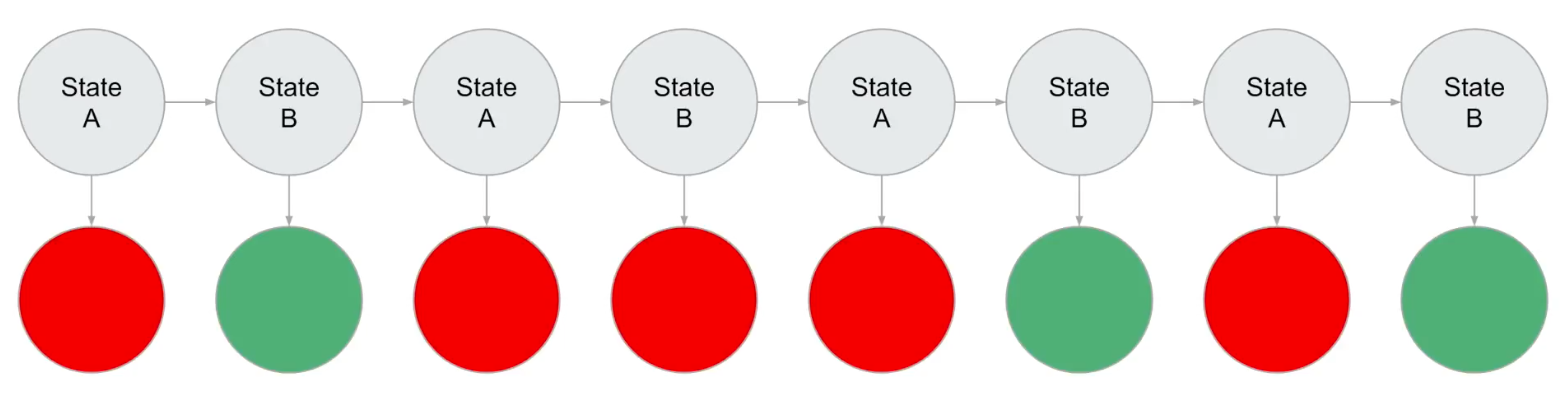
\includegraphics[scale=0.3]{hmm_example.png}
\caption{Visualization of a Hidden Markov Model. Upper circles represent hidden 
	states ($X_n$). Lower (colored) circles represent emitted observable states ($Y_n$)
	Adopted from \citep{hmm_figure}
	}
\label{fig:hmm}
\end{figure}

HMM is used to compute the likelyhood state sequences (often denoted
as \textit{hidden states}) of $X_n$ based on the 
observed sequence $Y_n$, conditional transition probability (often denoted
\textit{emission probability}) $P(Y_n \in A | X_n = x_n)$.
The Baum-Welch algorithm is used to fit the paramteres of the HMM based on the
observed data \citep{baggenstoss2001modified}. The Viterbi algorithm (described
in more detail in~\ref{sec:viterbi}) can be used to efficiently 
find the most likely sequence of hidden states based on 
the hidden state transition probabilities ($P(X_n | X_{n - 1})$,
emission probabilities ($P(Y_n | X_n)$), and initial state information $(P(X_1)$. 

HMM have been employed to model numerous tasks, such as 
speech recognition \citep{schuller2003hidden},
handwriting recognition, functional MRI brain mapping,  network anomaly
detection \citep{yu2010hidden} and many more.

\subsection{Viterbi algorithm}
\label{sec:viterbi}

The Viterbi algorithm is a recursive optimal solution to the problem of
estimating the state sequence of a discrete finite-state Markov process
\citep{howard1960dynamic} observed in memoryless noise
\citep{forney1973viterbi}. A Markov process is a stochastic process
whose future state values (time is discrete) are determined by
recent ones. Such a process generates a sequence of $T$ states 
$\textbf{x} = (x_0, \dots, x_T)$, where 
$x_t \in \{1, 2, \dots, K\}$, $\forall t \in {1, \dots, T}$
under the condition that :
$$
P(x_{t + 1} | x_0, x_1,\dots,x_t) = P(x_{t + 1} | x_t).
$$
Using the Viterbi algorithm it is then possible 
to find the most likley sequence of states -- 
the \textbf{Viterbi path}.

More formally, if we observe a sequence of
observations $\textbf{y} = (y_1, \dots, y_T)$ with output states
$y_i \in O = \{o_1, \dots, o_N\}$ with an initial state probability
probility array $\bm{\pi} = \{\pi_1,\dots, \pi_K\}$
behaving under a transition matrix $A$ of size $K \times K$
with element $A_ij$ storing the transition probability of
$s_i$ to $s_j$, 
and emission matrix $B$ of size $K \times N$ with 
element $B_ij$ storing probability of observing $o_j$ from $s_i$,
where $T$ is the number of steps, 
$K$ the number of possible states, and $N$ is the number of 
possible observations. We wish to find
$\textbf{x} = (x_1, \dots, x_T)$
as a sequence of states $x_i \in S = \{s_1, \dots, s_K\}$ 
most likely to generate the observed outputs under the 
conditions specified. 

A forward pass is made, which populates two
tables $T_1$ and $T_2$, both of size
$K \times T$. An element $T_1[i, j]$ stores 
probablities of the most likely path so far with 
$x_j = s_i$ that generates $\textbf{y} = (y_1, \dots, y_j)$.
$T_2[i, j]$ stores elements $x_{j - 1}$ of the most
likely path $\bm{\hat{x}} = (\hat{x}_1, \dots, \hat{x}_j = s_j)$:
\begin{align*}
T_1[i, j] = \max_k (T_1[k, j - 1] \cdot A_{ki} \cdot B_{iy_j}) \\
T_2[i, j] = \argmax_k (T_1[k, j - 1] \cdot A_{ki})
\end{align*}
calculated for each $k \in \{1, 2, \dots, K\}$, subsequence
of length $\forall j, 2 \leq j \leq T$

\subsection{Conditional Random Fields}
\label{sec:crf}

Conditional random fields (CRF) is a framework for building probablistic 
models to segment and label sequence data \citep{wallach2004conditional}
When trying to predict a vector $\mathbf{Y} = \{y_0, \dots, y_t\}$
of random variables given an observed feature vector 
$\mathbf{X} = \{x_0, \dots, x_t\}$. 
the typical supervised classification approach would be 
to learn independent classifiers to map $\forall i,  x \to y_i$
\citep{sutton2012introduction}.
However, this approach doesn't take into account possible dependencies
that may exist between labels, example being that neighboring 
regions in an image tend to have similar labels. 
Thus, predicting output variables can be represented as a graphical model.
Graphical models can be directed and undirected, but 
in the scope of this thesis, we limit ourselves to 
directed linear conditional random fields
and all subsequent definitions apply only to those. 
For an overview of other CRF, I recommend an
introductory, but comprehensive tutorial 
on CRFs \citep{sutton2012introduction} and the original paper on CRF by Lafferty et. al
\citep{lafferty2001conditional}. 

Formally, let $G = (V, E)$ be a graph such that $\mathbf{Y} = (\mathbf{Y}_v)_{v
\in V}$, so that $\mathbf{Y}$ is indexed by the vertices of $G$. Then
$(\mathbf{X}, \mathbf{Y}$) is a \textit{conditional random field} in case, when
conditioned on $\mathbf{X}$, the random variables $\mathbf{Y}_v$ obey the
Markov property with respect to the graph: $p(\mathbf{Y}_v | \mathbf{X},
\mathbf{Y}_w, w \neq v) = p(\mathbf{Y}_v | \mathbf{X}, \mathbf{Y}_w, w \sim v)$
, where $w \sim v$ means that $w$ and $v$ are neighbors in $G$
\citep{lafferty2001conditional}. 
For the linear chain case, $G$ is a simple chain
defined by: $G = (V = \{1, \dots, m\}, E = \{(i, i + 1)\})$, making 
$\mathbf{X} = (\mathbf{X_1}, \mathbf{X_2}, \dots, \mathbf{X_t})$
and $\mathbf{Y} = (\mathbf{Y_1}, \mathbf{Y_2}, \dots, \mathbf{Y_t})$.
%as depicted in figure~\ref{fig:chaincrf}. 
Now, the joint distribution of $X$ and $Y$ over $T$ time steps 
can be factorized as:
$$
p(x, y) = \prod_{t=1}^{T} p(y_t | y_{t - 1}) p(x_t | y_t)
$$
By setting $\theta_{ij} = \log p(y' = i | y = j)$ and
$\mu_{oi} = \log p(x = o | y = i)$ the joint distribution
can be rewritten as:
$$
p(x, y) = \frac{1}{Z} \prod_{t=1}^{T} exp \left\{ \sum_{i, j \in S} \theta_{ij} \mathbf{1}_{\{y_t=i\}} \mathbf{1}_{\{y_{t-1} = j\}}
+ \sum_{i \in S} \sum_{o \in O} \mu_{oi} \mathbf{1}_{\{y_t = i\}}\mathbf{1}_{\{x_t  = o\}} \right\}
$$
where $\theta = \{theta_{ij}, \mu_{oi}\}$ are parameters of the distribution and $Z$ is the
normalization constant. This can be shortened by 
introducing a \textit{feature function}
defined as $f_k (y_t, y_{t - 1}, x_t)$:
$$
p(x, y) = \frac{1}{Z} \prod_{t=1}^{T} exp \left\{ \sum_{k=1}^{K} \theta_k f_k(y_t, y_{t - 1}, x_t) \right\}
$$
Now, we can derive conditional distribution $p(y | x)$:
\begin{equation}\label{eq:cond_crf}
p(y | x) = \frac{p(y, x)}{\sum_{y'} p(y', x)}  = 
\frac{\prod_{t=1}^{T} exp \left\{ \sum_{k=1}^{K} \theta_k f_k(y_t, y_{t - 1}, x_t) \right\}}
{\sum_{y'} \prod_{t=1}^{T} exp \left\{ \sum_{k=1}^{K} \theta_k f_k(y'_t, y'_{t - 1}, x_t) \right\}}
\end{equation}
which is the definition of the \textit{linear-chain conditional random field}.
This definition can be extended such that the feature function can depend on 
multiple inputs, as the vector $x_t$ (representing all observations of $x$
until time step $t$) can be a parameter of the feature function $f_k$. 

Deriving inference in CRFs (finding 
$y^* = \argmax_y p(y | x)$) 
in the general case is intractable since 
it requires computing all possible $p(y_t, y_{t - 1} | x)$ 
and the normalizing constant $Z$, which grows exponentially with the 
sequence length. 
However, in the case of the linear-chain CRF it is possible to 
use dynamic-programming algorithms, such as the
forward-backward algorithm \citep{devijver1985baum} 
for computing the marginal distributions and 
the Viterbi algorithm
(section~\ref{sec:viterbi}) for computing
the most probable assignment. 
To estimate parameters $\theta$ of a conditional 
random field \textit{maximum likelyhood} is used.
A training dataset of $N$ samples $\{\mathbf{x}^{(i)}, \mathbf{y}^{(i)}\}^{N}_{i=1}$
where each $\mathbf{x}^{(i)} = \{x_{1}^{(i)}, \dots, x_{T}^{(i)}\}$
is a sequence of inputs
and $\mathbf{y}^{(i)} = \{y_{1}^{(i)}, \dots, y_{T}^{(i)}\}$ is 
a sequence of labels. To esimate parameters, we
minimize log likelyhood expressed as a function of parameters $\theta$:

$$
\theta^{*} = \argmin_{\theta} \sum_{i=1}^{N} \log p(\mathbf{y}^{(i)} | \mathbf{x}^{(i)} ; \theta)
$$
Expanding the conditional likelyhood using the definition of conditional random field
(equation~\ref{eq:cond_crf}) and adding an $L_2$ regularization factor $1/2 \sigma^2$ 
to penalize large weights:
$$
\sum_{i=1}^{N} \sum_{t=1}^{T} \sum_{k=1}^{K} \theta_k f_k (y_{t}^{(i)}, y_{t - 1}^{(i)} x_{t}^{(i)}) 
- \sum_{i=1}^N \log Z(x^{(i)}) - \sum_{k=1}^{K} \frac{\theta_{k}^{2}}{2 \sigma^2}
$$
Deriving to find the optimal set of $\theta$, we end up with:
$$
\frac{\partial }{\partial \theta_k} = \sum_{i=1}^{N} \sum_{t=1}^{T} f_k (y_{t}^{(i)}, y_{t - 1}^{(i)} x_{t}^{(i)}) 
- \sum_{i=1}^{N} \sum_{t=1}^{T} \sum_{y, y'} f_k (y, y', x_{t}^{(i)}) p(y, y'|x^{(i)}) - \frac{\theta_k}{\sigma^2}
$$
The result is a concave function (which is useful since we're looking for the 
maximum) since it is of the form $\log \sum_i \exp x_i$, thus can be optimized by
any hill climbing technique, with the 
Broyden-Fletcher-Goldfarb-Shanno algorithm \citep{liu1989limited} being a popular 
choice. 

CRFs, particularly linear-chain CRFs
have been widely applied in natural language processing in tasks such as
named entity recognition \citep{liu2011recognizing}, shallow parsing \citep{sha2003shallow}, 
extracting syntax from text \citep{taskar2004max}, 
semantic role labeling \citep{cohn2005semantic}, citation extraction \citep{wellner2004integrated}, 
sentiment analysis \citep{patra2014ju_cse} and many more. 

%TODO Applications of CRF
% Extracting syntax from natural-language text 

% \begin{figure}
% 	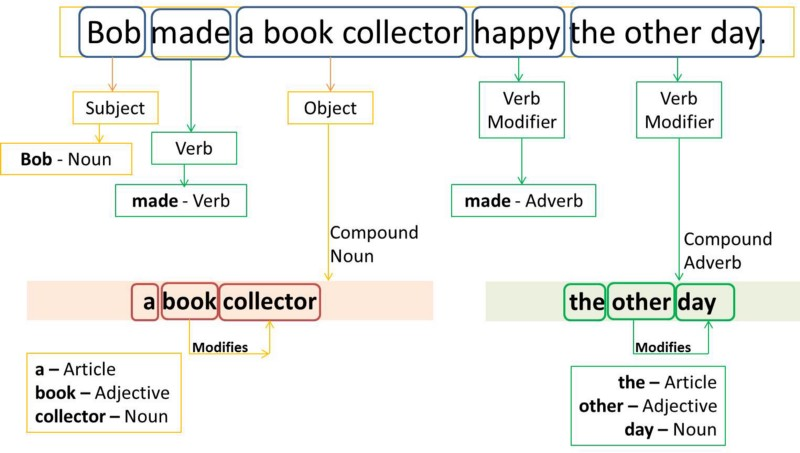
\includegraphics[scale=0.55]{pos_example.jpeg}
% \end{figure}
\begin{figure}
	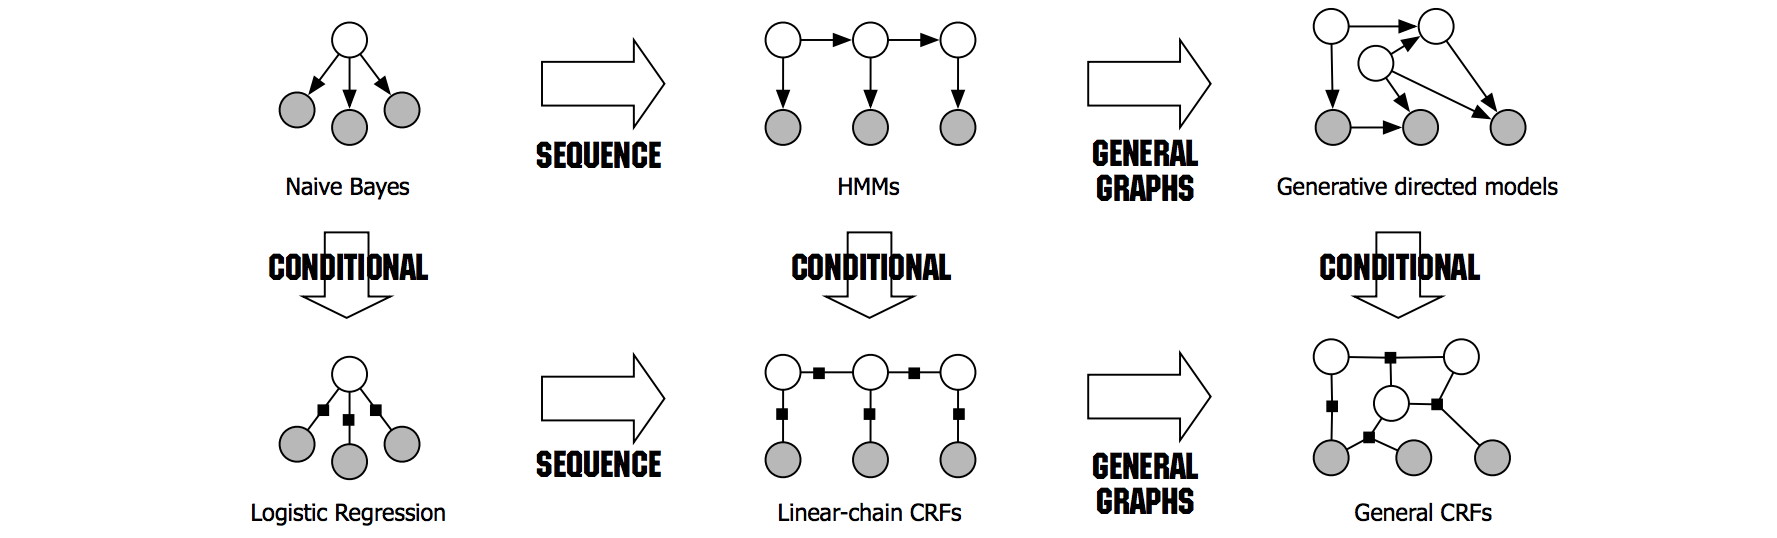
\includegraphics[width=\textwidth]{different_markovs.png}
	\caption{Visualization of differences between generative and discriminative approaches
	as well as sequential and non sequential approaches.
	Adopted from \citep{sutton2012introduction}}
	\label{fig:different_graphicals}
\end{figure}

% \begin{figure}
% 	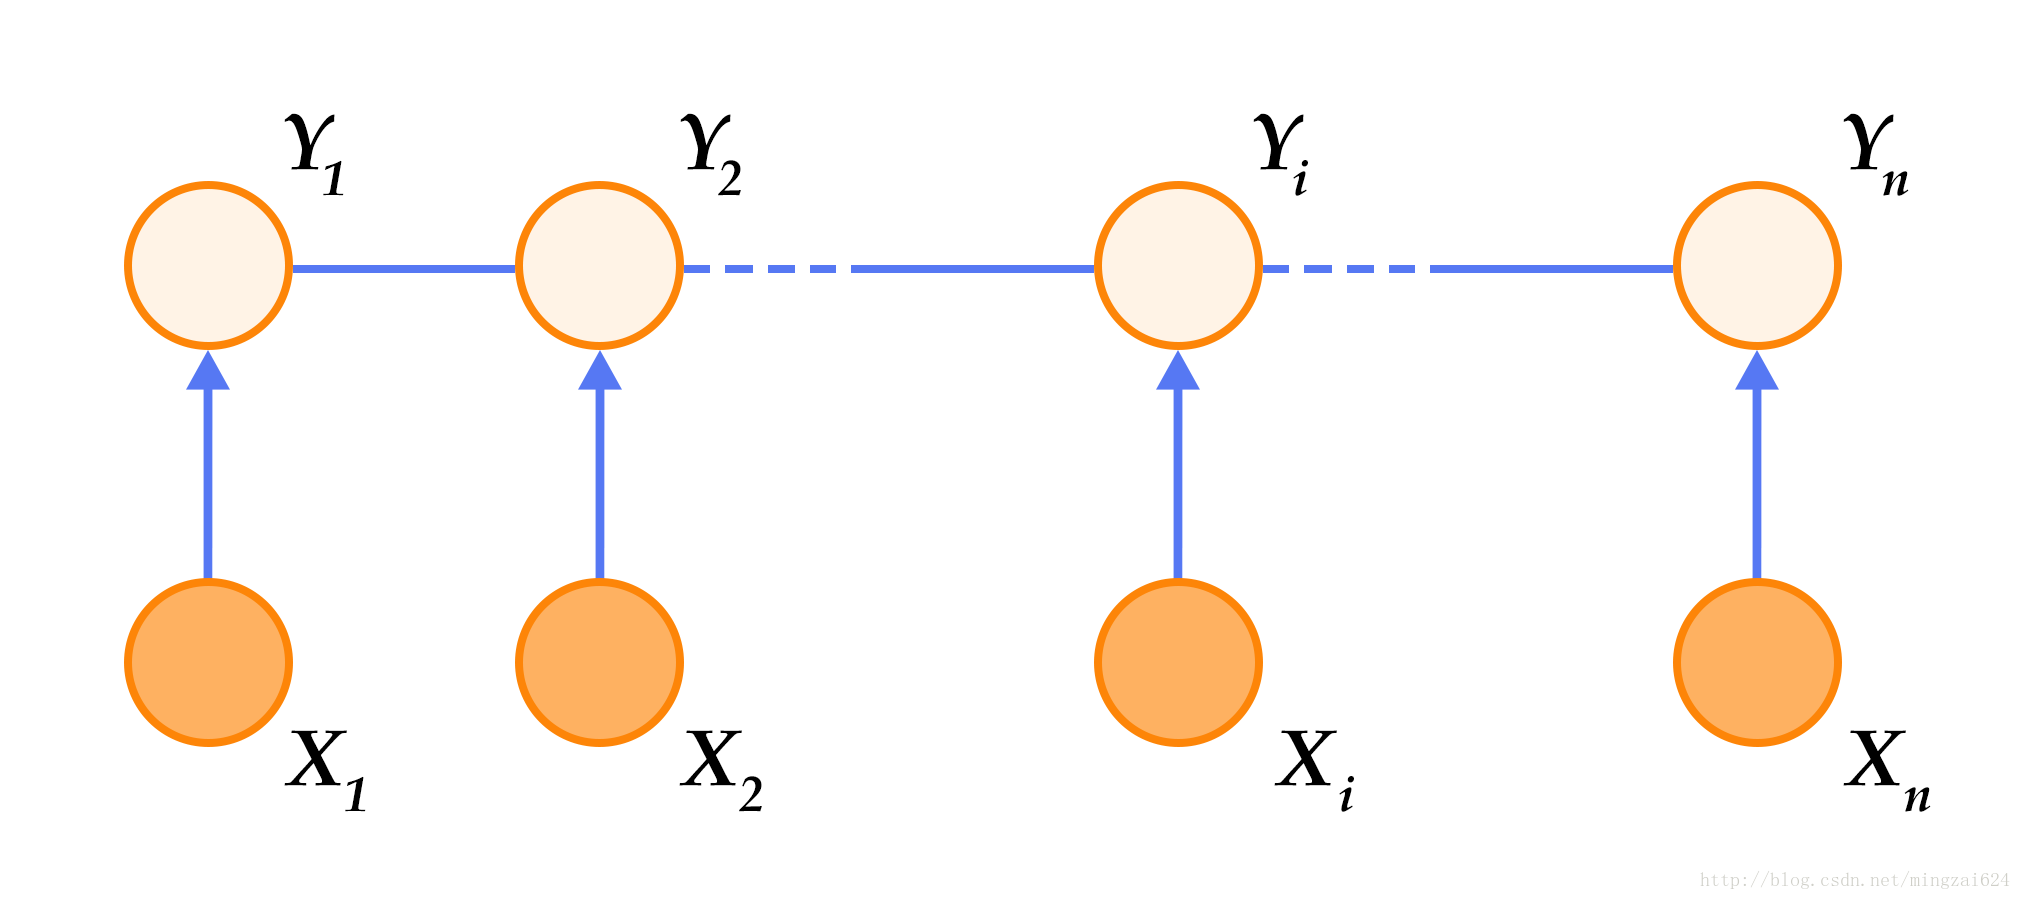
\includegraphics[scale=0.23]{chain_crf.png}
% 	\caption{Linear chain conditional random field \citep{chaincrffigure}}
% 	\label{fig:chaincrf}
% \end{figure}


\subsection{LSTM-CRF Model for Sequence Tagging}
\label{subsec:lstm_crf}

\begin{figure}
	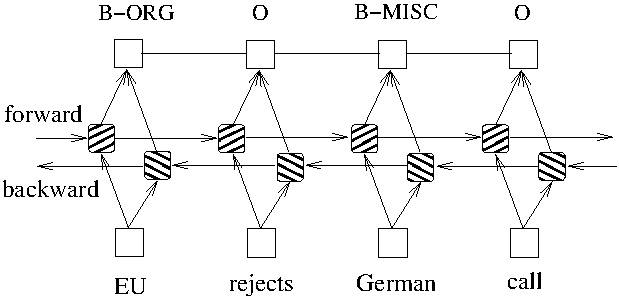
\includegraphics[width=0.8\textwidth]{biLstmCRF.pdf}
	\caption{A BiLSTM CRF model. Adopted from 
	\citep{huang2015bidirectional}
	}
	\label{fig:bilstm_crf}
\end{figure}


LSTM networks do a very good job of encoding sentences
(see section~\ref{sec:lstm}) to perform classification using only 
word embeddings as features (more on embeddings in section),
%TODO add reference
but do not take neighboring label information when performing sequence
classification which is important to solve sequence tagging
problems (such as named entity recognition \citep{nadeau2007survey}).
CRFs (see section~\ref{sec:crf}) allow for modeling label level 
dependencies and can work with arbitrary features, which have usually been
handcrafted.
Therefore, using an LSTM layer to encode words as features can be an input to a
CRF model which then uses standard 
parameter estimation to estimate its parameters. 
The combination of a bi-directional LSTM and a CRF is shown in figure~\ref{fig:bilstm_crf}.

CRF can use an arbitrary feature function $f_k$
to define its conditional probability (~\ref{eq:cond_crf}).
This feature function can 
be understood as the score of how well the sequence 
of states $y$ fit the given input $x$ and parameters $\theta$:
This score can be calculated as
:
$$
s_{LSTM-CRF}(x, y) = \sum_{t=0}^{T} \left( A_{t, t-1} + LSTM(x_t) \right)
$$
where $A$ is the transition matrix between states of $y$ with element
$A_{t, t-1}$ is the transition from state $y_{t-1}$ to state $y_{t}$, and $LSTM$
encodes input sentence using an LSTM network.
Dynamic programming methods (such as Viterbi~\ref{sec:viterbi}) can be used 
to efficiently compute optimal tag sequences
for inference. More details can be found in \citep{huang2015bidirectional}.

\subsection{Chain classification}
\label{sec:chain_classification}

Multilabel classification is a classification problem where 
a single instance may be assigned more than one class, making it 
a generalization of multiclass classification.
Formally, multiclass classification is the problem of finding 
a model that maps $x$ to binary vectors $y$, $y \in L = \{1, 2, \dots, N\}$. Typically, 
multilabel classification is usually framed as either:
\begin{enumerate}
	\item transformation into binary classification problems -- \textit{binary relevance} (BR) \citep{luaces2012binary} or
	\item transformation into multiclass problems \textit{label powerset} (LR).
\end{enumerate}
The binary relevance method transforms multilabel classification
into multiple binary problems; one problem for each label, such that each
binary model is trained to predict the relevance of one of the labels
\citep{read2011classifier}. This method trains $|L|$ binary classifiers
$C_1, \dots, C_{|L|}$ where each classifier $C_j$ predicts the $0/1$ association
for each correponding label $l_j \in L$ \citep{read2011classifier}.
Transforming from multi-label to binary with the BR method,
label correlations that might exist in training data are ignored, therefore
predicted labels might contain label combinations that might never occur in practice. 

\begin{figure}
\begin{algorithmic}[1]
\For{$j \in 1 \dots |L|$}
  \State $D' \gets \{\}$
	\For{$(x, S) \in D$}
	  \State $D' \gets D' \cup (x, l_1, \dots, l_{j - 1}, l_j)$
	  \State $C_j: D' \gets l_j \in \{0, 1\}$
	\EndFor
\EndFor
\end{algorithmic}
\caption{Classifier chain training phase for dataset 
	$D = \{(x_1, S_1), \dots, (x_n, S_n)\}$
	and label set $L$.
	Adopted from~\citep{read2011classifier}
	}

\label{alg:train_chain_classifier}
\end{figure}

\begin{figure}
\begin{algorithmic}[1]
\State $Y \gets \{\}$
\For{$j \in 1 \dots |L|$}
  \State $Y \gets Y \cup (l_j \gets C_j: (x, l_1, \dots, l_{j - 1})$
\EndFor
\Return $(x, Y)$
\end{algorithmic}
\caption{Classifier chain prediction phase for instance $x$ 
	and label set $L$.
	Adopted from~\citep{read2011classifier}
	}
\label{alg:test_chain_classifier}
\end{figure}

The label powerset method combines entire label sets into atomic labels 
to form a single-label problem for which the set of possible labels 
represents all distinct label subsets in the original multi-label 
representation. Each example $(x_i, S)$ is transformed into 
$(x_i, l)$, where $S$ represents the label combination set and
$l$ represents an atomic label representing the same combination set $S$
\citep{read2011classifier}. LR takes into 
consideration label correlations, but the number of combinations
is exponentially dependent on the number of labels $2^{|L|}$. 

The classifier chain method ($CC$) involves $|L|$ binary classifiers as in BM. 
Classifiers are chained such that each classifier deals with 
a single binary relevance problem $l_j \in L$ using an extended feature space of 
previous classifiers 
forming a chain of classifiers \citep{read2011classifier}.
The training phase is outlined in figure~\ref{alg:train_chain_classifier}. 
Each classifier $C_j$ in the chain is responsible for predicting 
the binary association of label $l_j$ using all prior 
binary relevance predictions in the chain $l_1, \dots, l_{j - 1}$.
The classification starts with $C_1$ determining 
$prediction(l_1 | x)$ propagating along the chain
to predict $prediction(l_j | x_i, l_1, \dots, l_{j-1})$, outlined 
in figure~\ref{alg:test_chain_classifier}
\citep{read2011classifier}.
The idea of the chaining method is to overcome the label independence problem
inherent to BM, retaining lower complexity advantages. 
For a more detailed complexity analysis see \citep{read2011classifier}. 
However, the ordering labels to train can have a significant effect on 
the classification accuracy. 

To overcome the ordering problems of classifier chains, one
can perform ensembling. 
Ensembling methods are learning algorithms 
that construct a set of classifiers and then classify new data 
points by taking a (weighted) vote of their predictions \citep{dietterich2000ensemble}.
Ensembling has proven to be succesful for multi-label 
problems, especially since it is usually easy to paralelize. 
\citep{tsoumakas2007random}. Classifier chains can also be
ensembled to try and overcome the ordering bias. An Ensemble 
Classifier Chain ($ECC$) trains $m$ chain classifiers training
each classifier with a random chain ordering (of $L$) and a random
subset of the dataset. Predictions of each  model $C_k, k \in \{1, \dots, m\}$ 
are then summed so that each label receives a number of votes
\citep{dimitriadou2001voting}.

\section{Unsupervised Machine Learning}
\label{sec:unsupervised_machine_learning}

As opposed to supervised machine learning (described in
section~\ref{sec:machine_learning}), unsupervised machine learning
has no access to labeled data. The goal of unsupervised machine learning,
often denoted as \textit{clustering} is to separate 
a finite unlabeled dataset into a finite and discrete set of 
\textit{natural} hidden data structures \citep{xu2005survey}.
Evaluating resulting clusters can be subjective, as there is a mere 
requirement that patterns in the same cluster should be similar to each
other, more than patterns in other clusters. More formally, 
given a set of input patterns $X = \{x_1, \dots, x_N\}$, where
$x_j = (x_{j1}, \dots, x_{jd})$ partitioning (clustering) can 
be performed in two ways \citep{xu2005survey}:
\begin{description}
\item[Hard clustering] seeks to partition $X$ into $K$ partitions $C=\{C_1, \dots, C_K\}, K \leq N$
	such that 
	\begin{enumerate}
	\item $C_i \neq \emptyset, i = 1, \dots, K$, 
	\item $\cup_{i=1}^{K} C_i = X$, and
	\item $C_i \cap C_j = \emptyset , i, j = 1, \dots K$ and $i \neq j$.
	\end{enumerate}
\item[Hierarchical clustering] constructs a tree-like partition of $X$ as 
	$H = \{H_1, \dots, H_Q\}, Q \leq N$ such that
	$C_i \in H_m, C_j \in H_n$ and $m > n$
	imply $C_i \in C_j$ or $C_i \cap C_j = \emptyset, \forall i, j, j \neq
		i, m = 1 \dots Q, l = 1 \dots Q$
\end{description}

\begin{figure}
	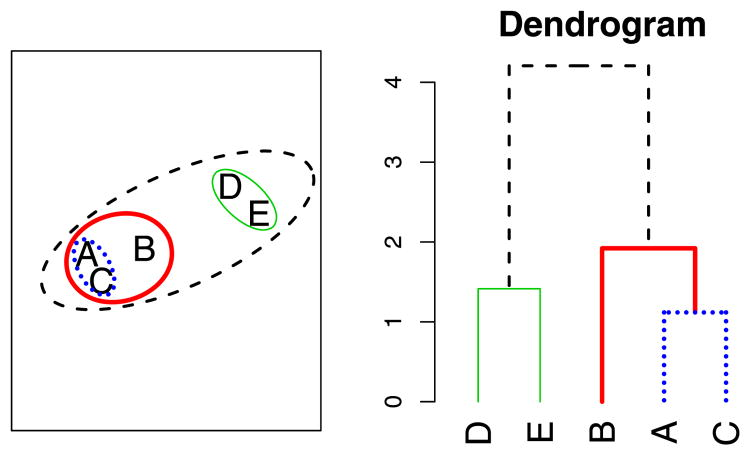
\includegraphics{clustering_linkage.jpg}
	\caption{
		Agglomerative hierarchical clustering produces a sequence of
		clusterings that can be represented as a dendrogram. Each
		interior node of the dendrogram corresponds to a merging of two
		clusters. Adopted from \citep{bien2011hierarchical}
	}

	\label{fig:clustering}
\end{figure}

\subsection{Hierarchical clustering}
\label{sec:hierarhical_clustering}

Hierarchical clustering is further subdivided into:
\begin{description}
	\item[Agglomerative]: a ``bottom-up'' approach where each observation
		starts in a single cluster and pairs of clusters are merged up the hierarchy and
	\item[Divisive]: a ``top-down'' approach where all observations start in one cluster on which
		splits are recursively performed down the hierarchy.
\end{description}
An example of agglomerative clustering is shown in figure~\ref{fig:clustering}. 
In order to determine which clusters should be combined (in the agglomerative case) or 
split (in the divisive case) there have to be defined measures of distance and a \textit{linkage 
criterion} which specifies the dissimilarity of clusters based on pairwise observation 
distances. Some common distance measures between two observations $a$ and $b$ are:
\begin{description}
	\item[Euclidan]: $||a - b||_2 = \sqrt{\sum_i (a_i - b_i)^2}$, 
	\item[Manhattan]: $||a - b||_1 = \sum_i |a_i - b_i|$, and
	\item[Maximum]: $||a - b||_{\infty} = \max_i |a_i - b_i|$.
\end{description}
and some common linkage criterion (according to \citep{szekely2005hierarchical}
between two clusters of observations $A$ and $B$ 
using distance metric $d$ are:
\begin{description}
	\item[Complete linkage]: $\max \{d(a, b): a \in A, b \in B\}$,
	\item[Minimum linkage]: $min \{d(a, b): a \in A, b \in B\}$,
	\item[Unweighted linkage]: $\frac{1}{|A| \cdot |B|} \sum_{a \in A} \sum_{b \in B} d(a, b)$,
	\item[Weighted average linkage]: $d(i \cup j, k) = \frac{d(i, k) + d(j, k)}{2}$, and
	\item[Ward's linkage] that minimizes the total within-cluster variance. It is calculated as
		$$
		\sum_{i \in A \cup B} ||x_i - m_{A \cup B}||^2 - \sum_{i \in A}||x_i - m_A||^2 
		- \sum_{i \in B} ||x_i - m_B||^2
		$$ 
		where $m_j$ is the center of cluster $j$  and $x_i$ is a datapoint
		in cluster $i$ \citep{ward1963hierarchical}.
\end{description}

% \citep{kaufman2009finding}
% \citep{reynolds2006clustering}

\subsection{Evaluation Methods}
\label{sec:clus_evaluation}

One standard way to evaluate the result of clustering is by
calculating the silhouette score \citep{reynolds2006clustering}. 
Let $C_M = \{C_1, \dots, C_k\}$ describe a clustering result, an 
exhaustive partitioning of dataset $D$. Then define the mean distance
between a single instance $i$ in cluster $C_i$ and all other points in the same cluster as
$$
a(i) = \frac{1}{|D_i| - 1} \sum_{j \in C_i, i \neq j} d(i, j)
$$
where $d(i, j)$ is the distance between data points $i$ and $j$ in
the cluster $C_i$. Then, define mean dissimilarity of an instance $i$ to
clusters it does not belong to $C \neq C_i$ as
$$
b(i) = \min_{k \neq i} \frac{1}{|C_k|} \sum_{j \in C_k} d(i, j)
$$.
Now, silhouette value of a single instance $i$ is defined as:
\begin{align}\label{eq:silhouette}
	s(i) &= \frac{b(i) - a(i)}{\max\{a(i), b(i)\}} \textrm{, if } |C_i| > 1 \\
	s(i) &= 0 \textrm{, if } |C_i| = 1
\end{align}
with $-1 \leq s(i) \leq 1$. Silhouette score close to $1$ means that a data point $i$
is very well matched with respect to the neighboring cluster, having large $a(i)$, whereas
having a large $b(i)$ makes silhouette score close to $-1$ implying that a data point is badly matched 
and it might be more appropriate to have it in the neighboring cluster. 
Silhouette score reflects how tightly grouped all data points in the cluster are
\citep{kaufman2009finding}.

\begin{table}
	\centering
	\begin{tabular}{c c c c c c c}
		\toprule
		Partition & & \multicolumn{4}{c}{$C$} & \\ \cline{3-6}
		& Group & $C_1$ & $C_2$ & \dots & $C_r$ & Total \\
		\midrule
		\multirow{4}{*}{$D$} & $D_1$ & $t_{11}$ & $t_{12}$ & \dots & $t_{1r}$ & $t_{1.}$ \\
		                     & $D_2$ & $t_{21}$ & $t_{22}$ & \dots & $t_{2r}$ & $t_{2.}$ \\
				     & $\vdots$ & $\vdots$ & $\vdots$ & $\ddots$ & $\vdots$ & $\vdots$ \\
		                     & $D_s$ & $t_{s1}$ & $t_{s2}$ & \dots & $t_{sr}$ & $t_{s.}$ \\
				     \midrule
		Total & &                      $t_{.1}$ & $t_{.2}$ & $\dots$&$t_{.r}$ & $t_{..} = N$ \\
				     \bottomrule
	\end{tabular}
	\caption{Adjusted rand index contigency table, adapted from \citep{santos2009use}}
	\label{tab:adjusted_rand}
\end{table}

\textit{Rand Index} is a measure of similarity between two clusters. \citep{santos2009use}
Given a dataset $X = \{x_1, \dots, x_N\}$ partitioned into two clustering results
$C = \{C_1, \dots, C_r\}$ and $D = \{D_1, \dots, D_s\}$ consisting of $r$ and $s$ clusters
respectively, define:
\begin{itemize}
\item $a$ as the number of pairs in $X$ that are in the same cluster in $C$ and $D$,
\item $b$ as the number of pairs in $X$ that are in different clusters in $C$ and $D$,
\item $c$ as the number of pairs in $X$ that are in the same clusters in $C$ and in different clusters of $D$, and
\item $d$ as the number of pairs in $X$ that are in different clusters in $C$ and in the same clusters in $D$. 
\end{itemize}
Rand index is then defined as:
\begin{equation}\label{eq:rand_index}
	R = \frac{a + b}{a + b + c + } = \frac{a + b}{\binom{n}{2}}
\end{equation}
where $a + b$ and $c + d$ reflects similarity and dissimilarity of two clusterings respectively.  
$\binom{n}{2}$ reflect the chance that two clusterings will randomly agree on a chosen pair. 
The Rand Index ($0 \leq R \leq 1$) value reflect how well two clusterings agree, with 
$0$ indicating complete disagremeent and $1$ signaling exactly same clusterings. 
\textit{Adjusted Rand Index} (ARI) is derived from Rand Index, but it is corrected for chance
\citep{steinley2004properties}. To calculate ARI, a contigency table is usually built which, 
given a dataset $X = \{x_1, \dots, x_N\}$ partitioned into two clustering
results $C = \{C_1, \dots, C_r\}$ and $D = \{D_1, \dots, D_s\}$ consisting of
$r$ and $s$ clusters, calculates the number of objects $n_{ij}$ common for every
$C_i$ and $D_j$, $t_{ij} = |C_i \cap D_j|$. Then row and column sums are calculated 
as shown in table~\ref{tab:adjusted_rand} using which ARI is calculated as:
\begin{equation}\label{eq:adjusted_rand_index}
	ARI = \frac{\sum_{ij} \binom{t_{ij}}{2}- \left[ \sum_i \binom{t_{i.}}{2} \sum_j \binom{t_{.j}}{2} \right] / \binom{N}{2}}
	{\frac{1}{2} \left[ \sum_i \binom{t_{i.}}{2} + \sum_j \binom{t_{.j}}{2} \right] - 
	\left[ \sum_i \binom{t_{i.}}{2} \sum_j \binom{t_{.j}}{2} \right] / \binom{N}{2}
	}
\end{equation}

\textit{V-measure} is an external entropy-based cluster evaluation measure which measures
how succesfully the criteria of homogeneity and completeness have been satisfied. 
\citep{rosenberg2007v}
It is computed as a harmonic mean of distinct homogeneity and completeness scores. 
\textit{Homogeneity} examines how close a given clustering $C = \{c_1, \dots, c_n\}$ of 
$N$ data points is to an ideal $K = \{k_1, \dots, k_m\}$ (members of a single
class should be in a single cluster) clustering by calculating the 
conditional entropy of the class distribution given the proposed clustering 
$H(C | K)$:
$$
h = 1 - \frac{H(C | K)}{H(C)}
$$
where 
\begin{align*} 
	H(C | K) &= - \sum_{k=1}^{|K|}\sum_{c=1}^{|C|} \frac{t_{ck}}{N}\log \frac{t_{ck}}{\sum_{c=1}^{|C|} t_{ck}} \\
	H(C) &= - \sum_{c=1}^{|C|} \frac{\sum_{k=1}^{K} t_{ck}}{n} \log \frac{\sum_{k=1}^{|K|} t_{ck}}{n}
\end{align*}
where $t_{ck}$ is a value in the contigency table between two clusterings as shown in table~
\ref{tab:adjusted_rand}.
To satisfy the \textit{completeness} criteria, a clustering must assign all 
members of a single class to a single class, making it symetrical to 
homogeneity, calculated through conditional entropy of the proposed clustering
given the class of datapoints $H(K | C)$:
$$
c = 1 - \frac{H(K | C)}{H(K)}
$$
where
\begin{align*}
H(K | C) &= - \sum_{c=1}^{|C|}\sum_{k=1}^{|K|} \frac{t_{ck}}{N} \log \frac{t_{ck}}{\sum_{k=1}^{|K|} t_{ck}} \\
H(K) &= - \sum_{k=1}^{|K|} \frac{\sum_{c=1}^{C} t_{ck}}{n} \log \frac{\sum_{c=1}^{|C|} t_{ck}}{n}
\end{align*}
where $t_{ck}$ is a value in the contigency table between two clusterings as shown in table~
\ref{tab:adjusted_rand}.
Now, through homogeneity $h$ and completeness $c$, we define V-measure as:
\begin{equation}\label{eq:v-measure}
	V = (1 + \beta) \cdot \frac{h \cdot c}{\beta \cdot h + c}
\end{equation}

% Adjusted Rand Index (ARI) (Hubertand Arabie, 1985) and the
% information-theoretic V-measure (Rosenberg and Hirschberg, 2007

\section{Natural Language Processing}
\label{sec:natural_language_processing}

Natural Language Processing (NLP) is a subfield of lingustics, computer
science, and artificial intelligence concerned with how to program computers to
process and analyze natural language data, text.  Natural Language Processing
techniques rely heavily on machine learning and statistical models which learn
from large amounts of textual data.  There are many subareas of natural
language processing, such as syntax, semantics, and discourse analysis.
Each of the subareas attempts to solve a set of problems, sentiment analysis, named
entity recognition, distributional semantics, recognizing textual entailment being
some of the problems of semantics. Good, yet comprehensive introductions to NLP are available 
in many books \citep{manning1999foundations} and review papers \citep{collobert2011natural}. 
Argumentation
mining is considered to closely related to natural language processing
\citep{lippi2015argument}, as it uses commonly used natural language processing
techniques to work on problems from social sciences to analyze arguments.
In the rest of this section, we give a introduction on various word representations
in subsections~\ref{sec:bow},~\ref{sec:tf-idf}, and~\ref{sec:embedding}, 
then we go into more detail on two 
semantics-related NLP problems: textual entailment in subsection~\ref{sec:textual_entailment}
and semantic textual similarity in subsection~\ref{sec:sts}.

\subsection{Bag-of-words}
\label{sec:bow}
In information retrieval it is often 
vital to efficiently 
store (index) and search collections of documents. 
To do so, documents are represented as features. 
One of the simplest document representations is applying the 
\textbf{bag-of-words} (BoW) model to text. BoW represents text as a multiset of
words along with their respective frequencies of occurence. However, it disregards
grammar and word order
\citep{harris1954distributional}, hence the term ``bag''. 
We show an example of calculating BoW
using an excerpt from \citep{dickens1949tale}:
\begin{quote}
``\emph{It was the best of times, \\
it was the worst of times, \\
it was the age of wisdom, \\
it was the age of foolishness,
}''
\end{quote}
We treat each line of the example as a document $D_i$ in the set of documents
$D$. The vocabulary $V$ is 
defined as all the unique words (ignoring case and punctuation)
across the document collection:
$$
V = \{t_{ij} | w_{ij} \in D_i \cap i \in \{1 \dots |D|\} \}
$$
For this example, the vocabulary amounts to
$V = \{$\emph{``it'', ``was'', ``the'' ``best'', ``of'', ``times'', ``worst'', ``age'',
``wisdom'', ``foolishness''}$\}$.
Now, for each word of the vocabulary, we calculate the frequency in the document. 
A BoW representation of document $D_4$ 
``\emph{it was the age of foolishness}''
would then be: $x_4 = [1, 1, 1, 0, 1, 0, 0, 1, 0, 1]$

The \textbf{n-gram} document recepresentation is a generalization of the BoW
approach. The ngram model
can use multiple words ($n$) to represent a document preserving some spatial information.
The bigram model ($n = 2$) uses pairs of words to represent a document
The document $D_4$ using a bigram model would then consist of:
\emph{``it was'', ``was the'', ``the age'', ``age of'', ``of foolishness''}.
BoW is a specialization of the ngram model
that sets $n=1$. 

The BoW model has been succesfully applied to many areas, such as language
modeling \citep{tirilly2008language}, sentiment analysis
\citep{wang2014microblog}, and spam classification \citep{kolari2006detecting}.
BoW models are
usually used with an assumption that similar documents have only similar
content. After transforming text into the BoW form, extra features can be
calculated, such as tf-idf or embedding features. 

\subsection{Tf-idf}
\label{sec:tf-idf}
%\label{sec:word_representations}
Some other commonly used features  to represent text are \textbf{term frequency
tf} and \textbf{inverse document frequency idf}. Term frequency of a word is
the number of occurences of that word in a given document:

$$
\mathit{tf}(t, d) = \frac{f(t, d)}{|d|}
$$
where $f(t, D_i)$ is the frequency of term (word) $t$ in document $D_i$ and $|D_i|$ is the number
of total terms in document $D_i$.
Inverse document frequency is a measure of how much information a word provides (common or rare
across a collection of documents) as is calculated as:

\begin{equation}
	\label{eq:idf}
\mathit{idf}(t, D) = \log \frac{N}{1 + |D_i \in D: t \in D_i|}
\end{equation}
where $N$ is the number of documents in the corpus $|D|$ and $|D_i \in D: t \in D_i|$ is the 
number of documents in which term $t$ appears in. 
These two features are often used together to represent a collection of documents 
$D_i \in D$ each containing a list of terms $t$:
$$
\mathit{tfidf} (t, D_i, D) = \mathit{tf}(t, D_i) \cdot \mathit{idf}(t, D)
$$
The vector space model \citep{meadow1992text} treats text documents as vectors  
in an $N$-dimensional space, where $N$ is the size of the vocabulary (total number of 
possible words). Comparing two documents in the vector space model can then be taking the
cosine similarity of the vectors features.

\subsection{Word embeddings}
\label{sec:embedding}

Another word representation approach represents each word using a fixed-size
vector of real numbers. A set of such approaches is called \textit{word
embeddings}. These vector representations of words are generated through
different methods, most popular two being neural networks and word co-occurence
matrix dimensionality reduction.

\begin{figure}
	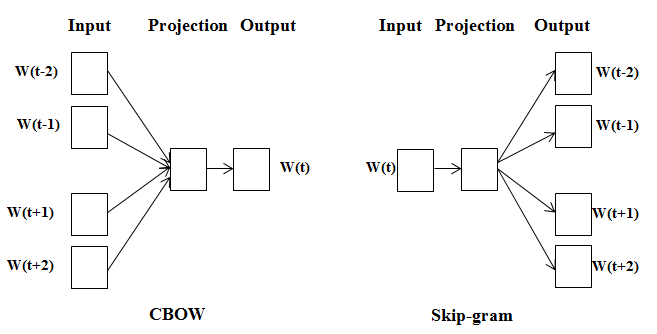
\includegraphics[scale=0.65]{skip_gram_cbow.png}
	\caption{CBOW (left) and skip-gram (right) simplified model architectures. Adopted from 
	\citep{suleiman2017deep}. }
	\label{fig:skip_gram_cbow}
\end{figure}

Word2vec is a neural network-based approach to generate distributed
representations of words \citep{mikolov2013distributed}.  It utilizes two
neural network models: a continuous \textit{bag-of-words} (CBOW) and continuous
\textit{skip-gram} approach.  The CBOW architecture is framed as a supervised
learning problem, where the model predicts the current word from a window of
surrounding context words. 
The ordering of the context words is not taken into
account (bag-of-words).  In the continuous skip-gram architecture, the model
uses the current word to predict the surrounding window of context words.
Architectures of both models are shown in figure~\ref{fig:skip_gram_cbow}. 
Models are then trained on large corpora, such as the Google Books corpus 
\citep{lin2012syntactic}. 
More details on training the models is available in the original word2vec papers
\citep{mikolov2013distributed, mikolov2013efficient}, as well as follow up papers
\citep{goldberg2014word2vec, rong2014word2vec}.
FastText is another word embedding procedure which is an extension on word2vec
\citep{bojanowski2017enriching}. In fastText each word is represented as a
n-gram of characters in order to capture the meaning of shorter words and allow
for embeddings to understand prefixes and suffixes. After splitting words into
subwords, similar procedures as the word2vec model are applied. 
The biggest advantage of using fastText is seen when dealing 
with rare words, which can be assigned a representation even if the word was
never seen during the model training period. 

\subsection{Textual Entailment}
\label{sec:textual_entailment}

\textit{Textual entailment} (TE) is defined as a directional relationship
between pairs of text expressions, denoted by $T$ --- the entailing ``Text'',
and $H$ --- the entailed ``Hypothesis''. We say that $T$ entails $H$ if,
typically, a human reading $T$ would infer that $H$ is most likely true 
\citep{dagan2005pascal}.  This definition assumes common human understanding of
language as well as common background knowledge. Examples of textual entailment
are in
table~\ref{tab:te_examples}.  
Recognizing textual entailment was established as
a popular natural language processing problem with the start of the
\textit{Recognising Textual Entailment} (RTE) challenge. The challenge involved
teams producing models to solve the TE problem on multiple datasets. A dataset
instance contained two sentences and a label whether entailment holds or not
($\mathit{True}$ or $\mathit{False}$).
Follow up challenges were organized \citep{bar2006second, giampiccolo2007third}.

\begin{table}
	\centering
	\begin{tabular}{p{8cm} | p{5cm} | c}
		Text & Hypothesis & TE \\
		\toprule
		\textit{
		Norway’s most famous painting, ``TheScream'' by Edvard Munch, was recov-ered
		Saturday, almost three months after it was stolen from an Oslo
		museum.} & 
		\textit{Edvard   Munch   painted ``The Scream''  }
		& $\mathit{True}$ \\
		\textit{Republic of Yemen is an Arab, Islamic and independent
		sovereign statewhose integrity is inviolable,  and  no part
		of which may be ceded.} & 
		\textit{The national language of Yemen is Arabic.}
		& $\mathit{True}$ \\
		\textit{Regan attended a ceremony in Washington to commemorate the
		landings in Normandy.} &
		\textit{Washington is located in Normandy. } & $\mathit{False}$ \\
		\bottomrule
	\end{tabular}
	\caption{Positive and negative examples of Textual Entailment (TE) 
	Adopted from \citep{dagan2005pascal}}
	\label{tab:te_examples}
\end{table}

Textual Entailment is closely related to the task of \textit{natural language inference} (NLI), 
where each pair of sentences can be assigned one of three possible labels:
\begin{enumerate*}
	\item entailment, 
	\item neutral, and
	\item contradiction. 
\end{enumerate*} 
making it more general than the TE challenge. 
The most used dataset of NLI is the Stanford Natural Language Inference dataset
\citep{bowman2015large} which contains 570K pairs of labelled sentence pairs. 
Examples of the dataset are available in table~\ref{tab:snli_examples}.

\begin{table}
	\centering
	\begin{tabular}{p{8cm} | p{5cm} | c}
		Text & Hypothesis & Relation \\
		\toprule
		\textit{
		A man inspects the uniform of a figure in some East Asian country.
		museum.} & 
		\textit{The man is sleeping}
		& $\mathit{Contradiction}$ \\
		\textit{An older and younger man smilling} & 
		\textit{Two men are smilling and laughing at the cats playing on the floor}
		& $\mathit{Neutral}$ \\
		\textit{A soccer game with multiple males playing} &
		\textit{Some men are playing a sport} & $\mathit{Entailment}$ \\
		\bottomrule
	\end{tabular}
	\caption{Positive and negative examples from the Standford Natural Language Inference dataset. 
	Adopted from \citep{bowman2015large}}
	\label{tab:snli_examples}
\end{table}

Some of the most successful attemps in solving NLI on the SNLI dataset have been
an enhanced LSTM model \citep{chen2016enhanced} and 
an attention based model \citep{parikh2016decomposable}. 
The enchanced LSTM model (basic LSTM described in section~\ref{sec:lstm}) 
uses an BiLSTM module to encode the text and hypothesis after which they calculate 
soft alignment between hidden representations of the text and hypothesis to model the
text--hypothesis interaction. Further, in parallel they use a Tree-LSTM to encode 
the text and hypothesis syntax trees and also compute soft alignment between them. 
Finally, they use a multilayer perceptron with $\mathit{tanh}$ activation and 
$\mathit{softmax}$ output after the alignment layers training the model end-to-end. 
At best, they achieve 88.6\% accuracy on the SNLI dataset. 
The attention-based approach \citep{parikh2016decomposable} first encodes 
text and hypothesis sentences as concatenations of word embeddings, upon which
soft alignment is computed using
neural attention. Then, the task is decomposed into separate problems (to optimize 
for training time) in which each aligned subphrases are compared (between the text and 
hypothesis). Finally, the computed subphrase alignments are aggregated in 
a standard feedforward layer to compute the label. They achieve 
86.8\% accuracy on the SNLI dataset. 

\subsection{Semantic Textual Similarity}
\label{sec:sts}

\textit{Semantic  Textual  Similarity}  (STS)  measures the  degree  of  semantic
equivalence  between two texts \citep{agirre2012semeval}. It is related to the problem
of Textual Entailment (TE). It assumes symmetric graded equivalence between
a pair of texts. STS is different from TE by incorporating the notion of 
graded semantic similarity, hence it is not a binary yes/no decision. 
STS is a unified framework built for 
extrinsic evaluation of multiple semantic components that otherwise
have tended to be evaluated in-dependently  and  without  broad
characterization  of their impact on NLP applications. 
Such components are word  sense  disambiguation, lexical  substitution,  semantic
role  labeling,  multi-word  expression  detection, discourse analysis, and 
many other. STS defines the similarity between two texts on a scale from 
0.0 (minimum similarity) to 4.0 (maximum similarity).

The most successful STS models from the SemEval-2012 relied on 
one of three approaches. The first uses information retrieval's 
vector space model \citep{meadow1992text} representing text in a 
``bag-of-words'' manner and then computing cosine similarity between 
resulting vectors. The second approach attempts to align words or expressions of
the sentence pair by maximizing the summation of word similarity \citep{mihalcea2006corpus}.
The third approach combines different measures and features which are then 
used as input to machine learning models fitted on such data 
\citep{vsaric2012takelab}. See \citep{han2013umbc_ebiquity}
for a more detailed overview. 

TakeLab's STS system by \citet{vsaric2012takelab} first preprocesses two input
texts (removing stopwords, hypens, slashes, \dots), after which they calculate
a set of syntactic, ngram overlap, and named entity features.  Finally, they
frame the problem as a supervised regression problem and train a LIBSVM
\citep{chang2011libsvm}, using grid search and cross-validation (described in
subsection~\ref{sec:selection}) to obtain optimal hyperparameters.

\section{Formal Knowledge Representation}
\label{sec:knowledge_representation}

Ontology defines a set of representational primitives with which to model 
a domain of knowledge or discourse. The primitives are classes, attributes
(or properties) and relationships (relations among class instances). 
Definitions of the primitives include information about their
meaning and constraints on their logically consistent application
\citep{gruber2009ontology}.
We discern between two basic types of ontologies: a domain ontology and an
upper ontology. 
Some core components of an ontology are:
\begin{description}
\item[Classes] sets, collections, concepts of kinds of things,
\item[Attributes] aspects, properties, features, distinguishable characteristics that
	individuals and classes can posses,
\item[Individuals] instances, objects that usually belong to a class,
\item[Relations] ways in which classes and individuals are related to each other,
\item[Axioms] assertions in a logical form that define the ontology for the domain of application, and
\item[Restrictions] formally stated descriptions that must be true for some assertion to be accepted. 
\end{description}

Domain ontology represents concepts which belong to a part of the world. 
They are used to model domain-specific definitions of terms. A single term is
unambiguous within a single domain ontology, but might be ambiguous across
different domain ontologies. For example, the term ``band'' can refer to a
medical band (like a bracelet used to track health-related metrics) in a
medical domain ontology, music band (musical ensemble which performs music) in
a composition domain ontology, or a rubber band (usually ring shaped loop of
rubber) in a toy domain ontology. Ontologies frequently change over time
when new requirements are added, the ontology is applied in different areas, different 
perceptions of the domain are needed \dots

\begin{figure}
	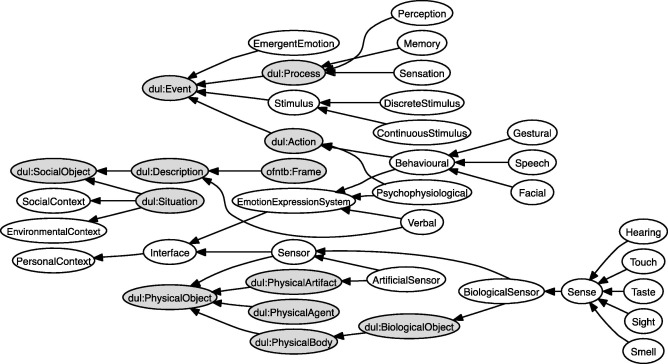
\includegraphics{upper_domain_interaction.jpg}
	\caption{An example of integrating a domain ontology
	(EmotionsOnto) with a upper ontology (DOLCE)
	Adopted from \citep{gil2015emotions}
	}
	\label{fig:upper_domain_integration}
\end{figure}

An upper ontology is a model of common relations and individuals that are generally
applicable across a wide range of domain ontologies. They usually have
a core glossary that contains terms and their decriptions of usage in various 
domain ontologies. Some popular upper ontologies are Dublin Core \citep{weibel1998dublin}, 
the suggested upper merged ontology SUMO \citep{pease2002suggested} and
DOLCE \citep{gangemi2002sweetening}. 
Upper ontologies are generally designed to be used with multiple domain ontologies. 
An example of an upper ontology integrated with a domain ontology is in 
figure~\ref{fig:upper_domain_integration}. 


% \begin{figure}
% 	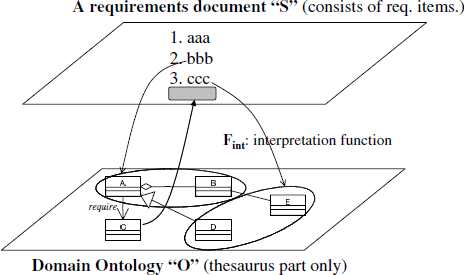
\includegraphics[scale=0.8]{ontology_creation.png}
% \end{figure}

Ontologies are often constructed from natural language requirements, 
such as ``a system can reserve seats in a specific train''. This sort of requirement can
then mapped to an ontological element ``reserve'' in the domain of 
reservation systems \citep{kaiya2006using}. 
Constructing a domain ontology often involves lexical decomposition
\citep{pustejovsky2013type} such that natural language requirements 
can be interpreted with ontological elements which can be decomposed 
into several unambiguous terms. The terms are often organized in a semantic structure,
a thesaurus of classes. Relationships between terms, relations, define how 
the terms are connected. 


% - (optional) joint modeling of sequence and classification \\
% 
% 
